\documentclass[tikz]{standalone}
% Curves the edge editor writes (M2b step 6). Each "coordinate" records a
% point on a curve, so the interpreter's control points can be checked
% against pdfTeX: bend left/right with and without an angle, out/in,
% looseness, separate out and in looseness, curves between anchors, a
% circle's border at an angle, and bends on "edge" operations.
\tikzset{every node/.style={draw, minimum width=1cm, minimum height=6mm}}
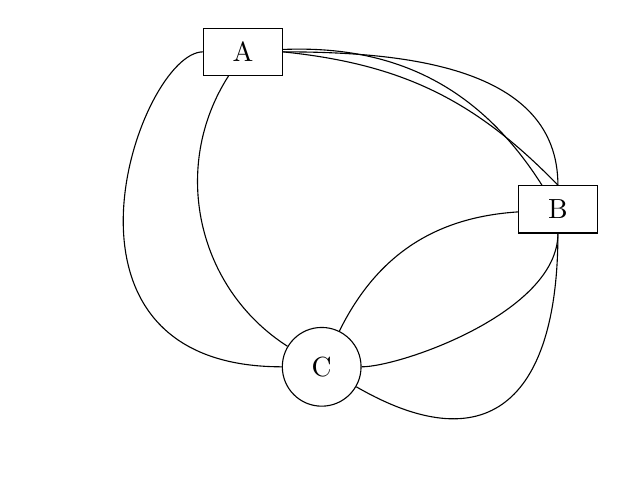
\begin{tikzpicture}
  \node (a) at (0,0) {A};
  \node (b) at (4,-2) {B};
  \node[circle] (c) at (1,-4) {C};
  \draw (a) to[bend left] coordinate[pos=0.25] (k1) coordinate[pos=0.5] (k2) (b);
  \draw (a) to[bend right=45] coordinate[pos=0.3] (k3) coordinate[pos=0.7] (k4) (c);
  \draw (b) to[out=90, in=0] coordinate[pos=0.25] (k5) coordinate[pos=0.6] (k6) (a);
  \draw (c) to[out=-30, in=-90, looseness=1.6] coordinate[pos=0.4] (k7) (b);
  \draw (a) to[out=180, in=180, out looseness=0.5, in looseness=2] coordinate[pos=0.3] (k8) coordinate[pos=0.8] (k9) (c);
  \draw (a.east) to[bend left=20] coordinate[pos=0.5] (k10) (b.north);
  \draw (c) edge[bend left] coordinate[pos=0.5] (k11) (b);
  \draw (b.south) .. controls +(0,-1) and +(1,0) .. coordinate[pos=0.5] (k12) (c);
\end{tikzpicture}
